\newcommand{\pashyasthitan}{{\Uchar"0CA4 \Uchar"0CCD \Uchar"0CB8 \Uchar"0CBF}\;\Uchar"0CCD \Uchar"0CA5}
ಮೊಟ್ಟ ಮೊದಲನೆಯ ಶ್ಲೋಕವೇ ನಮಗೆ ಚಿಂತನೆ, ಮನನ ಪ್ರಾರಂಭಿಸಲು ಬೇಕಾಗುವ ಸೂಕ್ಷ್ಮವಾದ ಸಂದೇಶವನ್ನು ಕೊಡುತ್ತದೆ.\\
\slcol{ಧೃತರಾಷ್ಟ್ರ ಉವಾಚ ।\\
\Index{ಧರ್ಮಕ್ಷೇತ್ರೇ ಕುರುಕ್ಷೇತ್ರೇ} ಸಮವೇತಾ ಯುಯುತ್ಸವಃ ।\\
ಮಾಮಕಾಃ ಪಾಂಡವಾಶ್ಚೈವ ಕಿಮಕುರ್ವತ ಸಂಜಯ ॥ ೧ ॥}
\cquote{ಧೃತರಾಷ್ಟ್ರನು ಹೇಳಿದನು,\\
ಸಂಜಯನೇ, ಯುದ್ಧದ ಬಯಕೆಯಿಂದ ಧರ್ಮಭೂಮಿಯಾದ ಕುರುಕ್ಷೇತ್ರದಲ್ಲಿ ಕಲೆತ ನನ್ನ ಮಕ್ಕಳೂ ಪಾಂಡವರೂ ಏನು ಮಾಡಿದರು?\\}
\slcol{ಸಂಜಯ ಉವಾಚ ।\\
\Index{ದೃಷ್ಟ್ವಾ ತು ಪಾಂಡವಾನೀಕಂ} ವ್ಯೂಢಂ ದುರ್ಯೋಧನಸ್ತದಾ ।\\
ಆಚಾರ್ಯಮುಪಸಂಗಮ್ಯ ರಾಜಾ ವಚನಮಬ್ರವೀತ್ ॥ ೨ ॥}
\cquote{ಸಂಜಯನು ಹೇಳಿದನು,\\
ಪಾಂಡವರ ದಂಡು ಸಜ್ಜಾಗಿ ನಿಂತಿದ್ದುದನ್ನು ನೋಡಿದ ಅರಸನಾದ ದುರ್ಯೋಧನನು ಗುರುಗಳಾದ ದ್ರೋಣರ ಬಳಿಗೆ ಬಂದು ಹೀಗೆ ಹೇಳಿದನು. \\}
\slcol{\Index{ಪಶ್ಯೈತಾಂ ಪಾಂಡುಪುತ್ರಾಣಾಮಾಚಾರ್ಯ} ಮಹತೀಂ ಚಮೂಮ್ ।\\
ವ್ಯೂಢಾಂ ದ್ರುಪದಪುತ್ರೇಣ ತವ ಶಿಷ್ಯೇಣ ಧೀಮತಾ ॥ ೩ ॥}
\cquote{ಗುರುಗಳೇ, ದೃಪದರಾಜನ ಮಗ ನಿಮ್ಮ ಶಿಷ್ಯ, ಬುದ್ಧಿಶಾಲಿಯಾದ ದೃಷ್ಟದ್ಯುಮ್ನ ಪಾಂಡವರ ಈ ದೊಡ್ಡ ದಂಡನ್ನು ಸಜ್ಜುಗೊಳಿಸಿರುವುದನ್ನು ನೋಡಿರಿ.\\}
\slcol{\Index{ಅತ್ರ ಶೂರಾ ಮಹೇಷ್ವಾಸಾ} ಭೀಮಾರ್ಜುನಸಮಾ ಯುಧಿ ।\\
ಯುಯುಧಾನೋ ವಿರಾಟಶ್ಚ ದ್ರುಪದಶ್ಚ ಮಹಾರಥಃ ॥ ೪ ॥}

\newpage
\newgeometry{margin=0pt} % Apply margin only for this page
\thispagestyle{empty}
\begin{figure}
\centering
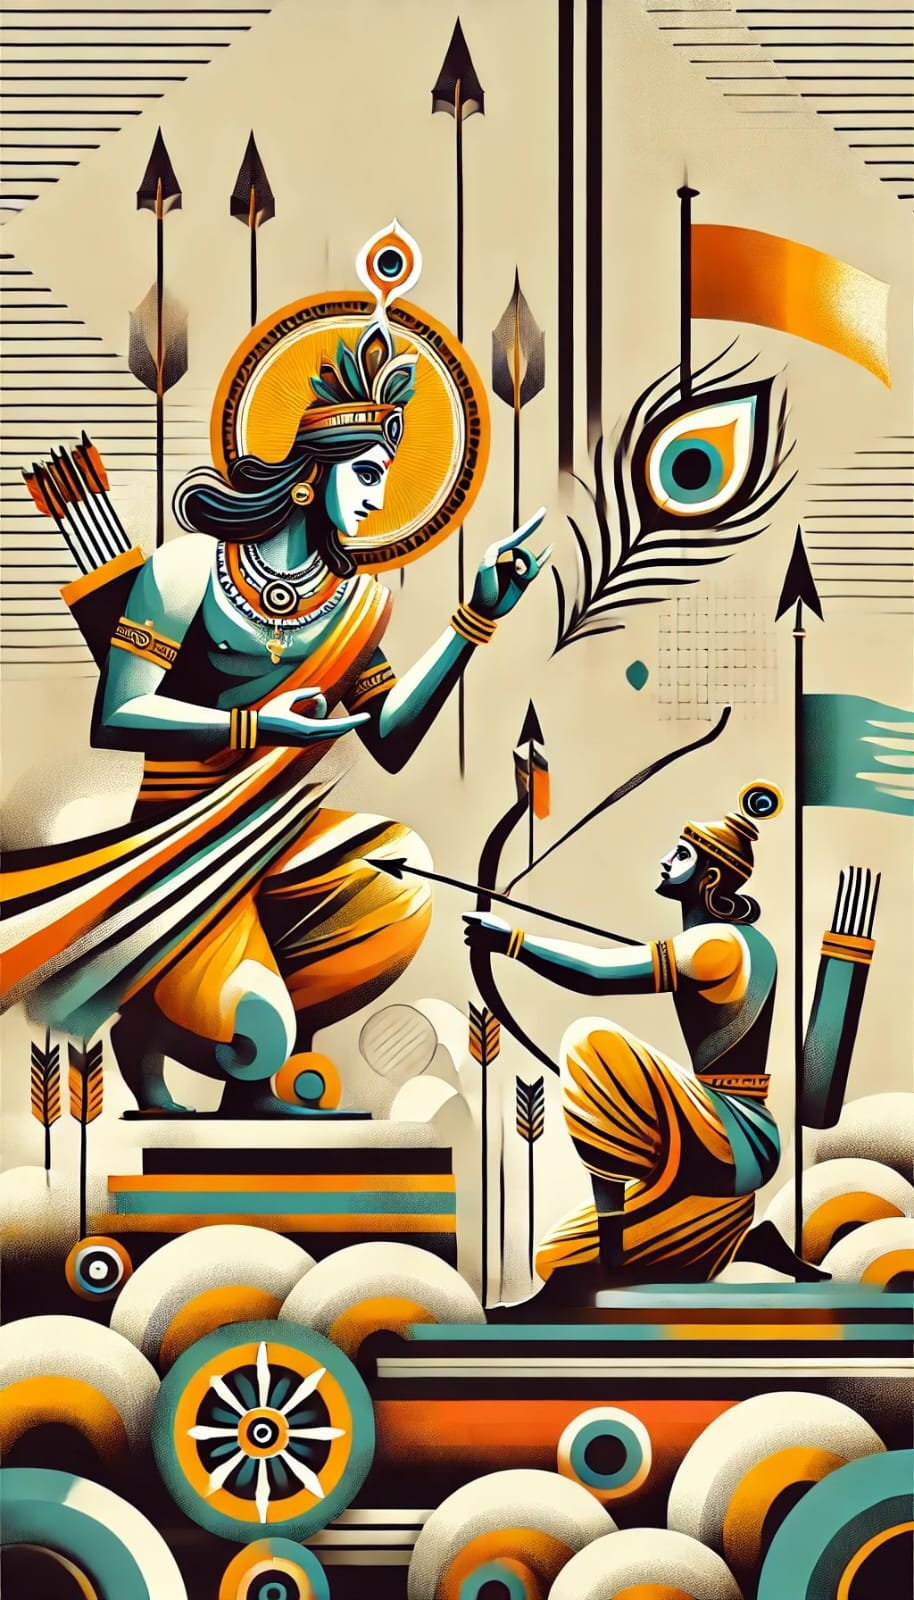
\includegraphics[width=\paperwidth, height=\paperheight]{./images/ArjunaVishada.jpg}
\end{figure}
\restoregeometry % Restore original geometry settings

\newpage
\begin{mananam}{\mananamfont ಮನನ ಶ್ಲೋಕ - ೧}
{\footnotesize \mananamtext ನನ್ನ ನಿತ್ಯ ಕರ್ಮದಲ್ಲಿ ದೇಹೆಂದ್ರೀಯ ಪ್ರವೃತ್ತಿಗಳಾದ ಆಸೆ, ಕೋಪ, ಭಯ, ಮತ್ಸರ ಇತ್ಯಾದಿಗಳೆಲ್ಲವನ್ನೂ ನನ್ನ ಅಂತರಂಗದಿಂದ ಪುಟ್ಟಿದೆದ್ದ, ತೀವ್ರತರ ಮುಕ್ತಿಯ ಹಂಬಲವು ಪ್ರತಿಭಟಿಸಿದಾಗ  ಇದಕ್ಕಾಗಿ, ಸನಾತನ ಗ್ರಂಥ ಮತ್ತು ಬೋಧಕರಿಂದ ಪಡೆದ ವಿವೇಕವನ್ನು ಅನುಸರಿಸಿದೆನೇ?(ದೇಹೇಂದ್ರೀಯ ಪ್ರವೃತ್ತಿಗಳನ್ನು ದಮನಿಸಲು)  ಯಾವ ಶಕ್ತಿ ಅಥವಾ ಮಾರ್ಗವನ್ನು ಅನುಸರಿಸಿದೆ?
ನನ್ನ ಶ್ರೇಷ್ಠವಾದ ಹಂಬಲ ಮತ್ತು ಸಂಕಲ್ಪಗಳನ್ನು ತಳ್ಳಿಹಾಕುವ ನನ್ನ ದುರಭ್ಯಾಸಗಳು ಮತ್ತು ಅಪಾಯಕಾರಿ ನಮೂನೆಗಳನ್ನು ನನ್ನ ನಿತ್ಯ ಜೀವನದ ಕದನದಲ್ಲಿ (ಜಂಝಾಟಗಳಲ್ಲಿ) ಗುರುತಿಸಬಲ್ಲೆನೇ?
}
\end{mananam}
\WritingHand\enspace\textbf{ಆತ್ಮ ವಿಮರ್ಶೆ}
\begin{inspiration}{\mananamfont ಸ್ಪೂರ್ತಿ}
{\footnotesize \mananamtext ನಿನ್ನಲ್ಲಿ ನೈಜಿಕತೆ (ಅಂದರೆ, ನಿನ್ನ ಮೌಲ್ಯಕ್ಕೆ ಅನುಗುಣವಾಗಿ ಬದುಕುವುದು) ಇರಲಿ,  ನೀನು ಉನ್ನತಿಯತ್ತ ಬದಲಾಗುವೆ.  ಪಕ್ಷಪಾತ ರಹಿತ ಅವಲೋಕನ, ಜೀವನ ಕೌಶಲ್ಯಕ್ಕೆ ಅತ್ಯಗತ್ಯ. ನಮ್ಮನ್ನು ನಾವು ಬದಲಾಯಿಸಿಕೊಳ್ಳಲು ಕೇವಲ ಬಯಕೆ ಇದ್ದರೆ ಮಾತ್ರ ಸಾಲದು, ಜ್ಞಾನಿಗಳ, ಋಷಿಗಳ ಮಹತ್ವದ ಉನ್ನತವಾದ ಬೋಧನೆಗಳಿಂದ ನಮ್ಮ ಯೋಚನೆಗಳು, ಮಾತುಗಳು ಮತ್ತು ಕೃತಿಗಳನ್ನು ತಹಬಂದಿಗೆ ತಂದು, ಪ್ರತಿದಿನವೂ ನಮ್ಮನ್ನು ನಾವು ಆತ್ಮ ವಿಮರ್ಶೆ ಮಾಡಿಕೊಳ್ಳಲೇಬೇಕು.}
\end{inspiration}
\newpage

\cquote{ಈ ದಂಡಿನಲ್ಲಿ ಹೋರಾಟದಲ್ಲಿ ಭೀಮಾರ್ಜುನರಿಗೆ ಸರಿ ಜೋಡಿಯಾದ ಶೂರರಾಗಿ ದೊಡ್ಡ ದೊಡ್ಡ ಬಿಲ್ಲುಗಳನ್ನು ಹಿಡಿದುಕೊಂಡು ಕಾದುವುದರಲ್ಲಿ ಕುಶಲರಾದ ಸಾತ್ಯಕಿ ವಿರಾಟರಿದ್ದಾರೆ. ಸಹಸ್ರ ಜನರೊಡನೆ ಏಕಾಂಗಿಯಾಗಿ ಹೋರಾಡಬಲ್ಲ ದ್ರುಪದನಿದ್ದಾನೆ.\\}
\slcol{\Index{ಧೃಷ್ಟಕೇತುಶ್ಚೇಕಿತಾನಃ} ಕಾಶಿರಾಜಶ್ಚ ವೀರ್ಯವಾನ್ ।\\
ಪುರುಜಿತ್ಕುಂತಿಭೋಜಶ್ಚ ಶೈಬ್ಯಶ್ಚ ನರಪುಂಗವಃ ॥ ೫ ॥}
\cquote{ದೃಷ್ಟಕೇತು, ಚೇಕಿತಾನ, ವೀರನಾದ ಕಾಶಿರಾಜ, ಮತ್ತು ಮನುಷ್ಯರಲ್ಲಿ ಶ್ರೇಷ್ಠನಾದ ಶೈಭ್ಯ ಇವರೆಲ್ಲ ಇದ್ದಾರೆ. \\} 
\slcol{\Index{ಯುಧಾಮನ್ಯುಶ್ಚ ವಿಕ್ರಾಂತ} ಉತ್ತಮೌಜಾಶ್ಚ ವೀರ್ಯವಾನ್ ।\\
ಸೌಭದ್ರೋ ದ್ರೌಪದೇಯಾಶ್ಚ ಸರ್ವ ಏವ ಮಹಾರಥಾಃ ॥ ೬ ॥}
\cquote{ಬಲಶಾಲಿಯಾದ ಯುಧಾಮನ್ಯು, ವೀರನಾದ ಉತ್ತಮೌಜ, ಸುಭದ್ರೆಯ ಮಗ ಅಭಿಮನ್ಯು ಮತ್ತು ದ್ರೌಪದಿಯ ಮಕ್ಕಳು ಇದ್ದಾರೆ. ಇವರೆಲ್ಲರೂ, ಒಬ್ಬೊಬ್ಬರೇ ಹತ್ತು ಸಹಸ್ರ ಜನರೊಡನೆ ಹೋರಾಡಬಲ್ಲ ಮಹಾರಥರು. \\}
\slcol{\Index{ಅಸ್ಮಾಕಂ ತು ವಿಶಿಷ್ಟಾ ಯೇ} ತಾನ್ನಿಬೋಧ ದ್ವಿಜೋತ್ತಮ ।\\
ನಾಯಕಾ ಮಮ ಸೈನ್ಯಸ್ಯ ಸಂಙ್ಞಾರ್ಥಂ ತಾನ್ಬ್ರವೀಮಿ ತೇ ॥ ೭ ॥}
\cquote{ಬ್ರಾಹ್ಮಣ ಶ್ರೇಷ್ಠರೇ, ನಮ್ಮ ಕಡೆಯಲ್ಲಿರುವ ವೀರರನ್ನು ನೆನಪಿಗೆ ತಂದುಕೊಳ್ಳಿ. ತಮಗೆ ನೆನಪಾಗಲೆಂದು ಅವರ ಹೆಸರುಗಳನ್ನು ಹೇಳುತ್ತೇನೆ.\\} 
\slcol{\Index{ಭವಾನ್ಭೀಷ್ಮಶ್ಚ ಕರ್ಣಶ್ಚ} ಕೃಪಶ್ಚ ಸಮಿತಿಂಜಯಃ ।\\
ಅಶ್ವತ್ಥಾಮಾ ವಿಕರ್ಣಶ್ಚ ಸೌಮದತ್ತಿಸ್ತಥೈವ ಚ ॥ ೮ ॥}
\cquote{ತಾವು ಭೀಷ್ಮ ಕರ್ಣ ಜಯಶೀಲನಾದ ಕೃಪಾ, ಅಶ್ವತ್ಥಾಮ, ವಿಕರ್ಣ ಸೋಮದತ್ತನ ಮಗನಾದ ಭೂರಿಶ್ರವ ಮತ್ತು ಜಯದ್ರಥ. \\}
\slcol{\Index{ಅನ್ಯೇ ಚ ಬಹವಃ} ಶೂರಾ ಮದರ್ಥೇ ತ್ಯಕ್ತಜೀವಿತಾಃ ।\\
ನಾನಾಶಸ್ತ್ರಪ್ರಹರಣಾಃ ಸರ್ವೇ ಯುದ್ಧವಿಶಾರದಾಃ ॥ ೯ ॥}
\cquote{ಇನ್ನೂ ಅನೇಕ ಶೂರರು ನನಗಾಗಿ ಜೀವ ತೆರಲು ಸಿದ್ದರಾಗಿ ಇದ್ದಾರೆ. ಎಲ್ಲರೂ ಎಲ್ಲಾ ಬಗೆಯ ಆಯುಧಗಳನ್ನು ಉಪಯೋಗಿಸಬಲ್ಲವರು ಮತ್ತು ಯುದ್ಧದಲ್ಲಿ ಗಟ್ಟಿಗರು.\\}
\slcol{\Index{ಅಪರ್ಯಾಪ್ತಂ ತದಸ್ಮಾಕಂ} ಬಲಂ ಭೀಷ್ಮಾಭಿರಕ್ಷಿತಮ್ ।\\
ಪರ್ಯಾಪ್ತಂ ತ್ವಿದಮೇತೇಷಾಂ ಬಲಂ ಭೀಮಾಭಿರಕ್ಷಿತಮ್ ॥ ೧೦ ॥}
\cquote{ಭೀಷ್ಮರ ರಕ್ಷಣೆಗೆ ಒಳಪಟ್ಟಿರುವ ನಮ್ಮ ದೊಡ್ಡ ಆ ದಂಡು ಸಾಲದೇನೋ ಎನಿಸುತ್ತದೆ. ಭೀಮನ ರಕ್ಷಣೆಗೆ ಒಳಪಟ್ಟಿರುವ ಪಾಂಡವರ ಈ ಸೇನೆ ಸಾಕಷ್ಟು ಸಮರ್ಥವಾಗಿದೆ.\\}
\slcol{\Index{ಅಯನೇಷು ಚ ಸರ್ವೇಷು} ಯಥಾಭಾಗಮವಸ್ಥಿತಾಃ ।\\
ಭೀಷ್ಮಮೇವಾಭಿರಕ್ಷಂತು ಭವಂತಃ ಸರ್ವ ಏವ ಹಿ ॥ ೧೧ ॥}
\cquote{ನೀವೆಲ್ಲರೂ ದಂಡಿನ ಬೇರೆ ಬೇರೆ ಮಾರ್ಗಗಳಲ್ಲಿ ನಿಮ್ಮ ನಿಮ್ಮ ಪಾಲಿಗೆ ಬಂದ ಕಡೆ ಇದ್ದುಕೊಂಡು ಭೀಷ್ಮರನ್ನು ರಕ್ಷಿಸಿರಿ.\\}
\slcol{\Index{ತಸ್ಯ ಸಂಜನಯನ್ಹರ್ಷಂ} ಕುರುವೃದ್ಧಃ ಪಿತಾಮಹಃ ।\\
ಸಿಂಹನಾದಂ ವಿನದ್ಯೋಚ್ಚೈಃ ಶಂಖಂ ದಧ್ಮೌ ಪ್ರತಾಪವಾನ್ ॥ ೧೨ ॥}
\cquote{ಹೀಗೆಂದು ಹೇಳಿದ ದುರ್ಯೋಧನನಿಗೆ ಹರ್ಷ ಉಂಟಾಗುವಂತೆ ಆಗ ಕುರುವಂಶದ ಹಿರಿಯ ಕೌರವರ ಅಜ್ಜ, ಪರಾಕ್ರಮಶಾಲಿ ಭೀಷ್ಮನು ಗಟ್ಟಿಯಾಗಿ ಸಿಂಹನಾದ ಮಾಡಿ ಶಂಖವನ್ನು ಊದಿದನು.\\}
\slcol{\Index{ತತಃ ಶಂಖಾಶ್ಚ ಭೇರ್ಯಶ್ಚ} ಪಣವಾನಕಗೋಮುಖಾಃ ।\\
ಸಹಸೈವಾಭ್ಯಹನ್ಯಂತ ಸ ಶಬ್ದಸ್ತುಮುಲೋऽಭವತ್ ॥ ೧೩ ॥}
\cquote{ಆಮೇಲೆ ಒಮ್ಮೆಲೆ ಶಂಖಗಳು, ಭೇರಿಗಳು, ಮೃದಂಗಗಳು, ನಗಾರಿಗಳು, ರಣಭೇರಿಗಳು  ಮೊಳಗಿದವು. ಆ ಗದ್ದಲವು ಎಲ್ಲೆಲ್ಲಿಯೂ ತುಂಬಿತು.\\}
\slcol{\Index{ತತಃ ಶ್ವೇತೈರ್ಹಯೈರ್ಯುಕ್ತೇ} ಮಹತಿ ಸ್ಯಂದನೇ ಸ್ಥಿತೌ ।\\
ಮಾಧವಃ ಪಾಂಡವಶ್ಚೈವ ದಿವ್ಯೌ ಶಂಖೌ ಪ್ರದಧ್ಮತುಃ ॥ ೧೪ ॥}
\cquote{ಆಮೇಲೆ ಬಿಳಿ ಕುದುರೆಯನ್ನು ಹೂಡಿದ ದೊಡ್ಡ ತೇರಿನ ಮೇಲೆ ಕುಳಿತಿದ್ದ ಕೃಷ್ಣನೂ ಅರ್ಜುನನೂ ಹೆಸರುವಾಸಿಯಾದ ದಿವ್ಯವಾದ ತಮ್ಮ ಶಂಖಗಳನ್ನು ಊದಿದರು.\\}
\slcol{\Index{ಪಾಂಚಜನ್ಯಂ ಹೃಷೀಕೇಶೋ} ದೇವದತ್ತಂ ಧನಂಜಯಃ ।\\
ಪೌಂಡ್ರಂ ದಧ್ಮೌ ಮಹಾಶಂಖಂ ಭೀಮಕರ್ಮಾ ವೃಕೋದರಃ ॥ ೧೫ ॥}
\cquote{ಕೃಷ್ಣನು ಪಾಂಚಜನ್ಯವನ್ನೂ ಅರ್ಜುನನು ದೇವದತ್ತವನ್ನೂ, ಶತ್ರುಗಳನ್ನು ಎದೆಗೂಡಿಸುವ ಭೀಮನು ಪೌಂಡ್ರವೆಂಬ ದೊಡ್ಡ ಶಂಖವನ್ನು ಊದಿದನು.\\}
\slcol{\Index{ಅನಂತವಿಜಯಂ ರಾಜಾ} ಕುಂತೀಪುತ್ರೋ ಯುಧಿಷ್ಠಿರಃ ।\\
ನಕುಲಃ ಸಹದೇವಶ್ಚ ಸುಘೋಷಮಣಿಪುಷ್ಪಕೌ ॥ ೧೬ ॥}
\cquote{ಕುಂತಿಯ ಹಿರಿಯ ಮಗ, ಅರಸನಾದ ಧರ್ಮರಾಯನು ಅನಂತ ವಿಜಯವನ್ನೂ ನಕುಲನು ಸುಘೋಷವನ್ನೂ ಸಹದೇವನು ಮಣಿಪುಷ್ಪಕವನ್ನೂ ಊದಿದರು. \\}
\slcol{\Index{ಕಾಶ್ಯಶ್ಚ ಪರಮೇಷ್ವಾಸಃ} ಶಿಖಂಡೀ ಚ ಮಹಾರಥಃ ।\\
ಧೃಷ್ಟದ್ಯುಮ್ನೋ ವಿರಾಟಶ್ಚ ಸಾತ್ಯಕಿಶ್ಚಾಪರಾಜಿತಃ ॥ ೧೭ ॥\\
\Index{ದ್ರುಪದೋ ದ್ರೌಪದೇಯಾಶ್ಚ} ಸರ್ವಶಃ ಪೃಥಿವೀಪತೇ ।\\
ಸೌಭದ್ರಶ್ಚ ಮಹಾಬಾಹುಃ ಶಂಖಾಂದಧ್ಮುಃ ಪೃಥಕ್ಪೃಥಕ್ ॥ ೧೮ ॥}
\cquote{ಓ ಧೃತರಾಷ್ಟ್ರ ಕೇಳು, ಹಿರಿಯ ಬಿಲ್ಲೋಜ ಕಾಶಿರಾಜ, ಮಹಾರಥನಾದ ಶಿಖಂಡಿ, ಧೃಷ್ಟದ್ಯುಮ್ನ,  ವಿರಾಟ, ಸೋಲರಿಯದ ಸಾತ್ಯಕಿ, ದ್ರುಪದ, ದ್ರೌಪದಿಯ ಮಕ್ಕಳು, ಮಹಾಬಾಹುವಾದ ಅಭಿಮನ್ಯು ಹೀಗೆ ಎಲ್ಲರೂ ತಮ್ಮ ತಮ್ಮ ಶಂಖಗಳನ್ನು ಊದಿದರು.\\}
\slcol{\Index{ಸ ಘೋಷೋ ಧಾರ್ತರಾಷ್ಟ್ರಾಣಾಂ} ಹೃದಯಾನಿ ವ್ಯದಾರಯತ್ ।\\
ನಭಶ್ಚ ಪೃಥಿವೀಂ ಚೈವ ತುಮುಲೋ ವ್ಯನುನಾದಯನ್ ॥ ೧೯ ॥}
\cquote{ಆ ಗದ್ದಲವು ಭೂಮಿಯಲ್ಲಿಯೂ ಆಕಾಶದಲ್ಲಿಯೂ ತುಂಬಿ ಪ್ರತಿಧ್ವನಿಯನ್ನು ಹಬ್ಬಿಸಿ ಕೌರವರ ಎದೆ ಬಿರಿಯುವಂತೆ ಮಾಡಿತು.\\}
\slcol{\Index{ಅಥ ವ್ಯವಸ್ಥಿತಾಂದೃಷ್ಟ್ವಾ} ಧಾರ್ತರಾಷ್ಟ್ರಾನ್ಕಪಿಧ್ವಜಃ ।\\
ಪ್ರವೃತ್ತೇ ಶಸ್ತ್ರಸಂಪಾತೇ ಧನುರುದ್ಯಮ್ಯ ಪಾಂಡವಃ ॥ ೨೦ ॥\\
\Index{ಹೃಷೀಕೇಶಂ ತದಾ} ವಾಕ್ಯಮಿದಮಾಹ ಮಹೀಪತೇ ।}
\cquote{ಓ ಧೃತರಾಷ್ಟ್ರ, ಸಜ್ಜಾಗಿ ಎದುರಿಗೆ ನಿಂತಿರುವ ಕೌರವರನ್ನು ನೋಡಿ ಕಪಿಧ್ವಜನಾದ ಅರ್ಜುನನು ಹೊಡೆದಾಟಕ್ಕೆ ಮೊದಲು ಮಾಡಬೇಕಾದ ಆ ಸಮಯದಲ್ಲಿ ಗಾಂಡೀವವನ್ನು ಕೈಗೆ ತೆಗೆದುಕೊಂಡು ಕೃಷ್ಣನನ್ನು ಕುರಿತು ಈ ಮಾತನ್ನು ಹೇಳಿದನು.\\}
\slcol{ಅರ್ಜುನ ಉವಾಚ ।\\
ಸೇನಯೋರುಭಯೋರ್ಮಧ್ಯೇ ರಥಂ ಸ್ಥಾಪಯ ಮೇऽಚ್ಯುತ ॥ ೨೧ ॥}
\cquote{ಅರ್ಜುನನು ಹೇಳಿದನು, ಕೃಷ್ಣ, ಎರಡು ದಂಡುಗಳ ನಡುವೆ ನನ್ನ ರಥವನ್ನು ನಿಲ್ಲಿಸು.\\}
\slcol{\Index{ಯಾವದೇತಾನ್ನಿರೀಕ್ಷೇऽಹಂ} ಯೋದ್ಧುಕಾಮಾನವಸ್ಥಿತಾನ್ ।\\
ಕೈರ್ಮಯಾ ಸಹ ಯೋದ್ಧವ್ಯಮಸ್ಮಿನ್ರಣಸಮುದ್ಯಮೇ ॥ ೨೨ ॥}
\cquote{ಕಾದಬೇಕೆಂದು ನಿಂತಿರುವವರನ್ನು, ಈ ಯುದ್ಧದಲ್ಲಿ ನಾನು ಯಾರೊಡನೆ ಕಾದಬೇಕಾಗಿದೆ ಎಂಬುದನ್ನು ಒಮ್ಮೆ ನೋಡುತ್ತೇನೆ.\\}
\slcol{\Index{ಯೋತ್ಸ್ಯಮಾನಾನವೇಕ್ಷೇऽಹಂ} ಯ ಏತೇऽತ್ರ ಸಮಾಗತಾಃ ।\\
ಧಾರ್ತರಾಷ್ಟ್ರಸ್ಯ ದುರ್ಬುದ್ಧೇರ್ಯುದ್ಧೇ ಪ್ರಿಯಚಿಕೀರ್ಷವಃ ॥ ೨೩ ॥}
\cquote{ದುರ್ಬುದ್ಧಿಯ ದುರ್ಯೋಧನನಿಗೆ ಈ ಯುದ್ಧದಲ್ಲಿ ನೆರವಾಗಬೇಕೆಂದು ಕಾದುವುದಕ್ಕಾಗಿ ಯಾರು ಯಾರು ಇಲ್ಲಿಗೆ ಬಂದಿರುತ್ತಾರೆ ಎಂಬುದನ್ನು ನಾನೊಮ್ಮೆ ನೋಡುತ್ತೇನೆ.\\}
\slcol{ಸಂಜಯ ಉವಾಚ ।\\
\Index{ಏವಮುಕ್ತೋ ಹೃಷೀಕೇಶೋ} ಗುಡಾಕೇಶೇನ ಭಾರತ ।\\
ಸೇನಯೋರುಭಯೋರ್ಮಧ್ಯೇ ಸ್ಥಾಪಯಿತ್ವಾ ರಥೋತ್ತಮಮ್ ॥ ೨೪ ॥\\
\Index{ಭೀಷ್ಮದ್ರೋಣಪ್ರಮುಖತಃ} ಸರ್ವೇಷಾಂ ಚ ಮಹೀಕ್ಷಿತಾಮ್ ।\\
ಉವಾಚ ಪಾರ್ಥ ಪಶ್ಯೈತಾನ್ಸಮವೇತಾನ್ಕುರೂನಿತಿ ॥ ೨೫ ॥}
\cquote{ಸಂಜಯನು ಹೇಳಿದನು,\\
ಧೃತರಾಷ್ಟ್ರನೇ, ಅರ್ಜುನನು ಹೀಗೆ ಹೇಳಿದಾಗ ಕೃಷ್ಣನು ಭೀಷ್ಮ ದ್ರೋಣರ ಮತ್ತು ಎಲ್ಲಾ ಅರಸರ ಎದುರಿಗೆ ಎರಡು ದಂಡುಗಳ ನಡುವೆ ರಥವನ್ನು ನಿಲ್ಲಿಸಿ ‘ಅರ್ಜುನನೇ ಇಲ್ಲಿ ನೆರೆದಿರುವರನ್ನು ನೋಡು’ ಎಂದು ಹೇಳಿದನು.\\}
\slcol{\Index{ತತ್ರಾಪಶ್ಯ\pashyasthitan ತಾನ್ಪಾರ್ಥಃ} ಪಿತೄನಥ ಪಿತಾಮಹಾನ್ ।\\
ಆಚಾರ್ಯಾನ್ಮಾತುಲಾನ್ ಭ್ರಾತೄನ್ ಪೌತ್ರಾನ್ ಸಖೀಂಸ್ತಥಾ ॥ ೨೬ ॥}
\cquote{ಅರ್ಜುನನು ಅಲ್ಲಿ ನಿಂತಿರುವ ಪಿತೃತುಲ್ಯರು, ಅಜ್ಜಂದಿರು, ಗುರುಗಳು, ಸೋದರ ಮಾವಂದಿರು, ಅಣ್ಣತಮ್ಮಂದಿರು, ಮಕ್ಕಳು, ಮೊಮ್ಮಕ್ಕಳು, ಜೊತೆಗಾರರು, ಮಾವಂದಿರು, ಸ್ನೇಹಿತರು- ಹೀಗೆ ಎಲ್ಲ ಬಗೆಯ ಬಂಧುಗಳನ್ನು ಎರಡು ಕಡೆಯ ದಂಡಿನಲ್ಲಿ ಕಂಡನು.\\}
\slcol{\Index{ಶ್ವಶುರಾನ್ಸುಹೃದಶ್ಚೈವ} ಸೇನಯೋರುಭಯೋರಪಿ ।\\
ತಾನ್ಸಮೀಕ್ಷ್ಯ ಸ ಕೌಂತೇಯಃ ಸರ್ವಾನ್ಬಂಧೂನವಸ್ಥಿತಾನ್ ॥ ೨೭ ॥}
\cquote{ಹೀಗೆ ಅಲ್ಲಿ ನೆರೆದಿರುವ ಬಂಧುಗಳನ್ನೆಲ್ಲ ನೋಡಿ ಅರ್ಜುನನು ತುಂಬಾ ಕನಿಕರಗೊಂಡು ವಿಷಾದದಿಂದ ಈ ಮಾತನ್ನು ಹೇಳಿದನು.\\}
\slcol{\Index{ಕೃಪಯಾ ಪರಯಾವಿಷ್ಟೋ} ವಿಷೀದನ್ನಿದಮಬ್ರವೀತ್ ।\\
ಅರ್ಜುನ ಉವಾಚ ।\\
ದೃಷ್ಟ್ವೇಮಂ ಸ್ವಜನಂ ಕೃಷ್ಣ ಯುಯುತ್ಸುಂ ಸಮುಪಸ್ಥಿತಮ್ ॥ ೨೮ ॥\\
\Index{ಸೀದಂತಿ ಮಮ ಗಾತ್ರಾಣಿ} ಮುಖಂ ಚ ಪರಿಶುಷ್ಯತಿ ।\\
ವೇಪಥುಶ್ಚ ಶರೀರೇ ಮೇ ರೋಮಹರ್ಷಶ್ಚ ಜಾಯತೇ ॥ ೨೯ ॥}
\cquote{ಅರ್ಜುನನು ಹೇಳಿದನು,\\
ಕೃಷ್ಣ, ಕಾದುವುದಕ್ಕೆ ಎಂದು ನೆರೆದಿರುವ ಈ ನನ್ನವರನ್ನು ನೋಡಿ ನನ್ನ ಅವಯವಗಳು ಸೊರುಗುತ್ತಿವೆ. ಬಾಯಿ ಒಣಗುತ್ತಿದೆ. ನನ್ನ ಮೈಯಲ್ಲಿ ನಡುಕ ಮೂಡಿ ರೋಮ ನಿಗುರಿ ನಿಂತಿದೆ.\\}
\slcol{\Index{ಗಾಂಡೀವಂ ಸ್ರಂಸತೇ} ಹಸ್ತಾತ್ತ್ವಕ್ಚೈವ ಪರಿದಹ್ಯತೇ ।\\
ನ ಚ ಶಕ್ನೋಮ್ಯವಸ್ಥಾತುಂ ಭ್ರಮತೀವ ಚ ಮೇ ಮನಃ ॥ ೩೦ ॥}
\cquote{ಕೈಯಿಂದ ಗಾಂಡೀವ ಧನುಸ್ಸು ಕುಸಿಯುತ್ತಿದೆ. ಚರ್ಮವು ಸುಡುತ್ತಿದೆ. ನನಗೆ ನಿಲ್ಲುವುದಕ್ಕೂ ಆಗುವುದಿಲ್ಲ. ನನ್ನ ಮನಸ್ಸು ತಳಮಳಗೊಂಡಿದೆ.\\}
\slcol{\Index{ನಿಮಿತ್ತಾನಿ ಚ ಪಶ್ಯಾಮಿ} ವಿಪರೀತಾನಿ ಕೇಶವ ।\\
ನ ಚ ಶ್ರೇಯೋऽನುಪಶ್ಯಾಮಿ ಹತ್ವಾ ಸ್ವಜನಮಾಹವೇ ॥ ೩೧ ॥}
\cquote{ಕೃಷ್ಣ, ಕೆಟ್ಟ ಅಪಶಕುನಗಳನ್ನು ಕಾಣುತ್ತಿದ್ದೇನೆ. ಯುದ್ಧದಲ್ಲಿ ನನ್ನವರನ್ನು ಕೊಂದರೆ ಒಳ್ಳೆಯದಾದೀತೆಂದು ನನಗೆ ಅನ್ನಿಸುವುದಿಲ್ಲ.\\}
\slcol{\Index{ನ ಕಾಂಕ್ಷೇ ವಿಜಯಂ ಕೃಷ್ಣ} ನ ಚ ರಾಜ್ಯಂ ಸುಖಾನಿ ಚ ।\\
ಕಿಂ ನೋ ರಾಜ್ಯೇನ ಗೋವಿಂದ ಕಿಂ ಭೋಗೈರ್ಜೀವಿತೇನ ವಾ ॥ ೩೨ ॥}
\cquote{ಕೃಷ್ಣ, ನನಗೆ ಗೆಲ್ಲುವ ಬಯಕೆ ಇಲ್ಲ. ನನಗೆ ರಾಜ್ಯವು ಬೇಡ, ಸುಖಗಳೂ ಬೇಡ. ಗೋವಿಂದ, ಇಂಥ ರಾಜ್ಯದಿಂದಾಗಲಿ ಭೋಗದಿಂದಾಗಲಿ ಬದುಕಿನಿಂದಲೆ ಆಗಲಿ ಏನು ಪ್ರಯೋಜನ?\\}

\newpage
\newgeometry{margin=0pt} % Apply margin only for this page
\thispagestyle{empty}
\begin{figure}
\centering
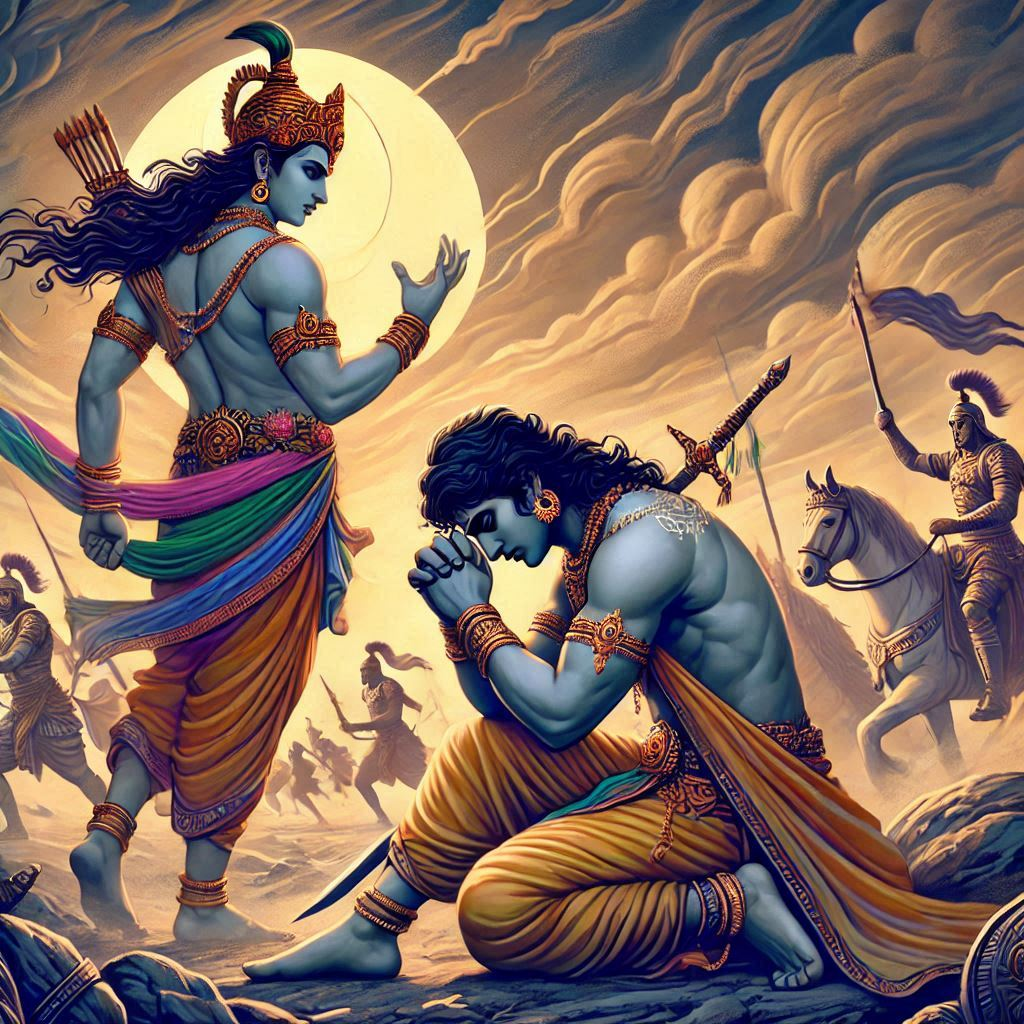
\includegraphics[width=\paperwidth, height=\paperheight]{./images/Arjuna2.png}
\end{figure}
\restoregeometry % Restore original geometry settings

\newpage
\begin{mananam}{\mananamfont ಮನನ  ಶ್ಲೋಕ - ೨೮ ೨೯ ೩೦}
{\footnotesize \mananamtext  ಹೊರಗಿನ ಸನ್ನಿವೇಶಗಳಿಂದಾಗಿ,  ಕೈಮೀರಿದ  ಮತ್ತು ಬುದ್ಧಿ ಭ್ರಮಿಸುವಂತಹ ನನ್ನ ಜೀವನದಲ್ಲಿಯ ಭಯಂಕರವಾದ ಉದ್ವೇಗಗಳನ್ನು ಎದುರಿಸಿದ ಸಂದರ್ಭಗಳನ್ನು ಪರ್ಯಾಲೋಚಿಸುತ್ತೇನೆ; ನನ್ನ ಜೀವನದ ಅಂತಹ ಸಂದರ್ಭಗಳಲ್ಲಿ ನನ್ನ ಮಾನಸಿಕ ಭಯಗಳಿಂದಾಗಿ ನನ್ನ ದೈಹಿಕ ಸ್ಥಿತಿ ಕುಂಠಿತವಾಯಿತೆಂಬುದನ್ನು ನಾನು ಅರಿತಿದ್ದೇನೆಯೇ? ನಾನು ನನ್ನ ಜೀವನದಲ್ಲಿನ ಉದ್ವೇಗ ಮತ್ತು ಭಯವನ್ನು ಹೇಗೆ ಎದುರಿಸಬಲ್ಲೆ?}
\end{mananam}
\WritingHand\enspace\textbf{ಆತ್ಮ ವಿಮರ್ಶೆ}
\begin{inspiration}{\mananamfont ಸ್ಪೂರ್ತಿ}
{\footnotesize \mananamtext ನಿಮ್ಮ ಯೋಚನೆಗಳ ಬಗ್ಗೆ ಎಚ್ಚರದಿಂದಿರಿ. ನಿಮ್ಮ ಮಾನಸಿಕ ಸ್ಥಿತಿ ನಿಮ್ಮ ದೇಹದ ಮೇಲೆ ಪರಿಣಾಮ ಬೀರುತ್ತದೆ. ಪ್ರತಿನಿತ್ಯದ ಒತ್ತಡದಿಂದ ಮನಸ್ಸನ್ನು ಸ್ವಾತಂತ್ರ್ಯಗೊಳಿಸಲು ಕೆಲವು ಸರಳ ಯೋಗದ ಮತ್ತು ಉಸಿರಾಟದ ಪ್ರಕ್ರಿಯೆಗಳು ಸಹಕಾರಿಯಾಗುತ್ತವೆ.}
\end{inspiration}
\newpage

\slcol{\Index{ಯೇಷಾಮರ್ಥೇ ಕಾಂಕ್ಷಿತಂ} ನೋ ರಾಜ್ಯಂ ಭೋಗಾಃ ಸುಖಾನಿ ಚ ।\\
ತ ಇಮೇऽವಸ್ಥಿತಾ ಯುದ್ಧೇ ಪ್ರಾಣಾಂಸ್ತ್ಯಕ್ತ್ವಾ ಧನಾನಿ ಚ ॥ ೩೩ ॥}
\cquote{ಯಾರಿಗಾಗಿ ನಾವು ರಾಜ್ಯವನ್ನೂ ಭೋಗಗಳನ್ನೂ ಸುಖಗಳನ್ನೂ ಬಯಸಿದೆವೋ, ಆ ಜನರೆಲ್ಲ ಜೀವದಾಸೆಯನ್ನೂ ಸಿರಿಯನ್ನೂ ತೊರೆದು ಇಲ್ಲಿ ಕಾದುವುದಕ್ಕೆ ನಿಂತಿದ್ದಾರೆ.\\}
\slcol{\Index{ಆಚಾರ್ಯಾಃ ಪಿತರಃ} ಪುತ್ರಾಸ್ತಥೈವ ಚ ಪಿತಾಮಹಾಃ ।\\
ಮಾತುಲಾಃ ಶ್ವಶುರಾಃ ಪೌತ್ರಾಃ ಶ್ಯಾಲಾಃ ಸಂಬಂಧಿನಸ್ತಥಾ ॥ ೩೪ ॥}
\cquote{ಗುರುಗಳು, ಪಿತೃತುಲ್ಯಯರು, ಮಕ್ಕಳು, ಅಜ್ಜಂದಿರು, ಸೋದರ ಮಾವಂದಿರು, ಮಾವಂದಿರು, ಮೊಮ್ಮಕ್ಕಳು, ಭಾವ ಮೈದುನರು, ಅದರಂತೆ ಬೇರೆ ಬೇರೆ ಸಂಬಂಧವುಳ್ಳವರು ಇಲ್ಲಿ ಎದುರು ನಿಂತಿದ್ದಾರೆ.\\}
\slcol{\Index{ಏತಾನ್ನ ಹಂತುಮಿಚ್ಛಾಮಿ} ಘ್ನತೋऽಪಿ ಮಧುಸೂದನ ।\\
ಅಪಿ ತ್ರೈಲೋಕ್ಯರಾಜ್ಯಸ್ಯ ಹೇತೋಃ ಕಿಂ ನು ಮಹೀಕೃತೇ ॥ ೩೫ ॥}
\cquote{ಕೃಷ್ಣ, ಅವರಿಂದ ನಾನು ಸತ್ತರೂ ಸರಿ. ಮೂರು ಲೋಕಗಳೇ ದೊರೆಯುವುದೆಂದರೂ ಇವರನ್ನು ಸಾಯಿಸಲಾರೆ. ಇನ್ನು ಈ ನೆಲಕ್ಕಾಗಿ ಹೊಡೆದೇನೆ?\\}
\slcol{\Index{ನಿಹತ್ಯ ಧಾರ್ತರಾಷ್ಟ್ರಾನ್ನಃ} ಕಾ ಪ್ರೀತಿಃ ಸ್ಯಾಜ್ಜನಾರ್ದನ ।\\
ಪಾಪಮೇವಾಶ್ರಯೇದಸ್ಮಾನ್ಹ{{ತ್ವೆ}\;\char"0CD6}ತಾನಾತತಾಯಿನಃ ॥ ೩೬ ॥}
\cquote{ಕೃಷ್ಣ, ಕೌರವರನ್ನು ಕೊಂದು ನಮಗೇನು ತೃಪ್ತಿ? ಈ ಕೇಡಿಗಳನ್ನು ಕೊಲ್ಲುವುದರಿಂದ ನಮಗೆ ಪಾಪವೇ ಗಂಟುಬಿದ್ದೀತು.\\}
\slcol{\Index{ತಸ್ಮಾನ್ನಾರ್ಹಾ ವಯಂ ಹಂತುಂ} ಧಾರ್ತರಾಷ್ಟ್ರಾನ್ಸ್ವಬಾಂಧವಾನ್ ।\\
ಸ್ವಜನಂ ಹಿ ಕಥಂ ಹತ್ವಾ ಸುಖಿನಃ ಸ್ಯಾಮ ಮಾಧವ ॥ ೩೭ ॥}
\cquote{ಆದ್ದರಿಂದ ನಮ್ಮವರಾದ ಕೌರವರನ್ನು ನಾವು ಕೊಲ್ಲಬಾರದು, ಮಾಧವ ನಮ್ಮವರನ್ನೇ ಕೊಂದು ನಾವು ಹೇಗೆ ಸುಖಿಗಳಾಗಿರುವೆವು?\\}
\slcol{\Index{ಯದ್ಯಪ್ಯೇತೇ ನ ಪಶ್ಯಂತಿ} ಲೋಭೋಪಹತಚೇತಸಃ ।\\
ಕುಲಕ್ಷಯಕೃತಂ ದೋಷಂ ಮಿತ್ರದ್ರೋಹೇ ಚ ಪಾತಕಮ್ ॥ ೩೮ ॥}
\cquote{ಆಸೆಗೆ ಬಲಿಯಾಗಿ ಬುದ್ಧಿ ಕಳಕೊಂಡ ಈ ಜನ ಕುಲನಾಶದ ಕೆಟ್ಟ ಪರಿಣಾಮವನ್ನೂ ಗೆಳೆಯರಿಗೆ ಮೋಸ ಮಾಡಿದ ಪಾಪವನ್ನೂ ಅರ್ಥಮಾಡಿಕೊಳ್ಳುತ್ತಿಲ್ಲ, ನಿಜ.\\}
\slcol{\Index{ಕಥಂ ನ ಜ್ಞೇಯಮಸ್ಮಾಭಿಃ} ಪಾಪಾದಸ್ಮಾನ್ನಿವರ್ತಿತುಮ್ ।\\
ಕುಲಕ್ಷಯಕೃತಂ ದೋಷಂ ಪ್ರಪಶ್ಯದ್ಭಿರ್ಜನಾರ್ದನ ॥ ೩೯ ॥}
\cquote{ಆದರೆ ಓ ಜನಾರ್ದನ, ಕುಲನಾಶದ ದುರಂತವನ್ನು ತಿಳಿದ ನಮಗೆ ಈ ಪಾಪದಿಂದ ಹಿಮ್ಮೆಟ್ಟಬೇಕೆಂದು ತಿಳಿಯದಿರುವುದು ಹೇಗೆ? \\}

\newpage
\begin{mananam}{\mananamfont ಮನನ ಶ್ಲೋಕ - ೩೭}
{\footnotesize \mananamtext ಯಾವ ಸಮಯದಲ್ಲಾದರೂ ಜವಾಬ್ದಾರಿಯ ಕೊರತೆಯಿಂದಾಗಿ ನಾನು ನನ್ನ ಕ್ರಿಯೆ ಮತ್ತು ನಿಷ್ಕ್ರಿಯೆಗಳನ್ನು ಸಮರ್ಥಿಸಿಕೊಂಡಿದ್ದೇನೆಯೇ? ಪೊಳ್ಳು ಅರ್ಥದ ಅನುಕಂಪದಿಂದ ನನ್ನನ್ನು ಅಧ್ಯಾತ್ಮದಿಂದ ಕೆಳಗೆ ತಳ್ಳುವವರು ಮತ್ತು ಋಣಾತ್ಮಕವಾಗಿ ಪ್ರಭಾವ ಬೀರುವವರಿಂದ ಸಂಬಂಧ ಕಡಿದುಕೊಳ್ಳುವ ಭಯ ನನಗಿದೆಯೇ? ನನ್ನ ಆಧ್ಯಾತ್ಮಿಕ ಜೀವನಕ್ಕೆ ಉಪಯೋಗವಿಲ್ಲದ ಜನರಿಗೆ ಮತ್ತು ಆಹ್ವಾನಕ್ಕೆ "ಇಲ್ಲ" ಅಥವಾ "ಬೇಡ" ಎಂದು ಹೇಳಲಾರದಷ್ಟು ದುರ್ಬಲನೆ ನಾನು?}
\end{mananam}
\WritingHand\enspace\textbf{ಆತ್ಮ ವಿಮರ್ಶೆ}
\begin{inspiration}{\mananamfont ಸ್ಪೂರ್ತಿ}
{\footnotesize \mananamtext ಜೀವನದ ಸ್ಪರ್ಧೆಗಳನ್ನು ಎದುರಿಸಿ ನಿಲ್ಲಬೇಕು. ನಾವೇ ಸ್ವತಃ ನಮ್ಮ ಜೀವನಕ್ಕಾಗಿ ಜವಾಬ್ದಾರರಾಗಿರಬೇಕು.  ನಿಷ್ಕಾರುಣ್ಯವಾಗಿ, ಎಲ್ಲಾ ಋಣಾತ್ಮಕ ಸಹವಾಸಗಳಿಂದ ಮತ್ತು ಪರಿಸರಗಳಿಂದ ದೂರವಾಗಿರಬೇಕು. ಇನ್ನೊಬ್ಬರ ಕೈಯಿಂದ ನಿಮ್ಮ ಮಾನಸಿಕ ನೆಮ್ಮದಿಯನ್ನು ಕಳೆದುಕೊಳ್ಳುವಂತಹದರ ಬಗ್ಗೆ ರಾಜಿ ಮಾಡಿಕೊಳ್ಳಬಾರದು. ಭೂತಕಾಲವನ್ನು ಹೋಗಲು ಬಿಡಬೇಕು ಮತ್ತು ವರ್ತಮಾನದಲ್ಲಿ ಉತ್ತಮವಾದದ್ದನ್ನು ಮಾಡಬೇಕು. ಅಂದರೆ, ಹಳೆಯ ಮತ್ತು ಮನಸ್ಸನ್ನು ಉದಾಸೀನಗೊಳಿಸುವ, ಆಗು, ಹೋಗುಗಳನ್ನು ಮರೆತು, ಉತ್ಸಾಹದಿಂದ ದೈನಂದಿನ ಕಾರ್ಯಗಳಲ್ಲಿ ತೊಡಗಿಸಿಕೊಳ್ಳಬೇಕು; ಹಾಗಾದಾಗ,  ಉತ್ತಮವಾದ ಭವಿಷ್ಯ ನಿಮ್ಮದೇ ಹಿಡಿತದಲ್ಲಿರುವುದು.}
\end{inspiration}
\newpage

\slcol{\Index{ಕುಲಕ್ಷಯೇ ಪ್ರಣಶ್ಯಂತಿ} ಕುಲಧರ್ಮಾಃ ಸನಾತನಾಃ ।\\
ಧರ್ಮೇ ನಷ್ಟೇ ಕುಲಂ ಕೃತ್ಸ್ನಮಧರ್ಮೋऽಭಿಭವತ್ಯುತ ॥ ೪೦ ॥}
\cquote{ಕುಲ ನಾಶವಾದರೆ ಬಹು ಕಾಲದಿಂದ ನಡೆದು ಬಂದ ಕುಲ ಧರ್ಮಗಳೆಲ್ಲ ಹೋಗಿ ಬಿಡುವುವು. ಕುಲಧರ್ಮ ಹಾಳಾದರೆ ಕುಲವನ್ನೆಲ್ಲ ಅಧರ್ಮವು ಆಕ್ರಮಿಸಿ ಬಿಡುವುವು.\\}
\slcol{\Index{ಅಧರ್ಮಾಭಿಭವಾತ್ಕೃಷ್ಣ} ಪ್ರದುಷ್ಯಂತಿ ಕುಲಸ್ತ್ರಿಯಃ ।\\
ಸ್ತ್ರೀಷು ದುಷ್ಟಾಸು ವಾರ್ಷ್ಣೇಯ ಜಾಯತೇ ವರ್ಣಸಂಕರಃ ॥ ೪೧ ॥}
\cquote{ಕೃಷ್ಣ, ಅಧರ್ಮದ ಆಕ್ರಮಣದಿಂದ ಕುಲೀನ ಹೆಂಗಸರು ಕೆಡುವರು. ಹೆಂಗಸರು ಕೆಟ್ಟರೆ ವರ್ಣಸಂಕರವು ಏರ್ಪದುತ್ತದೆ. \\}
\slcol{\Index{ಸಂಕರೋ ನರಕಾಯೈವ} ಕುಲಘ್ನಾನಾಂ ಕುಲಸ್ಯ ಚ ।\\
ಪತಂತಿ ಪಿತರೋ ಹ್ಯೇಷಾಂ ಲುಪ್ತಪಿಂಡೋದಕಕ್ರಿಯಾಃ ॥ ೪೨ ॥}
\cquote{ಇಂತಹ ಬೆರಕೆಯ ಸಮಾಜ ಕುಲವನ್ನು ಕುಲಕಂಠಕರನ್ನೂ ಜನತೆಯನ್ನು ನರಕಕ್ಕೆ ತಳ್ಳುತ್ತದೆ. ಅದರಿಂದ ಇಂಥವರಿಂದ ಹಿರಿಯರು ಪಿಂಡಪ್ರದಾನ, ಜಲತರ್ಪಣ ಇಲ್ಲದವರಾಗಿ ಕೆಳಕ್ಕೆ ಬೀಳುವರು.\\}
\slcol{\Index{ದೋಷೈರೇತೈಃ ಕುಲಘ್ನಾನಾಂ} ವರ್ಣಸಂಕರಕಾರಕೈಃ ।\\
ಉತ್ಸಾದ್ಯಂತೇ ಜಾತಿಧರ್ಮಾಃ ಕುಲಧರ್ಮಾಶ್ಚ ಶಾಶ್ವತಾಃ ॥ ೪೩ ॥}
\cquote{ಸಮಾಜದ ವ್ಯವಸ್ಥೆಯನ್ನು ಕೆಡಿಸುವ ಇಂತಹ ಈ ಕುಲನಾಶಕರ ದೋಷಗಳಿಂದಾಗಿ ನಿರಂತರವಾಗಿ ನಡೆದು ಬಂದ ಜಾತಿಧರ್ಮಗಳೂ ಕುಲ ಧರ್ಮಗಳೂ ನಿರ್ಮೂಲವಾಗುತ್ತವೆ.\\}
\slcol{\Index{ಉತ್ಸನ್ನಕುಲಧರ್ಮಾಣಾಂ} ಮನುಷ್ಯಾಣಾಂ ಜನಾರ್ದನ ।\\
ನರಕೇऽನಿಯತಂ ವಾಸೋ ಭವತೀತ್ಯನುಶುಶ್ರುಮ ॥ ೪೪ ॥}
\cquote{ಜನಾರ್ದನ, ಕುಲಕರ್ಮಗಳನ್ನೆಲ್ಲ ಹಾಳು ಮಾಡಿಕೊಂಡ ಮನುಷ್ಯರು ಯಾವಾಗಲೂ ನರಕದಲ್ಲಿರಬೇಕಾಗುವುದೆಂದು ಕೇಳಿದ್ದುಂಟು.\\}
\slcol{\Index{ಅಹೋ ಬತ ಮಹತ್ಪಾಪಂ} ಕರ್ತುಂ ವ್ಯವಸಿತಾ ವಯಮ್ ।\\
ಯದ್ರಾಜ್ಯಸುಖಲೋಭೇನ ಹಂತುಂ ಸ್ವಜನಮುದ್ಯತಾಃ ॥ ೪೫ ॥}
\cquote{ರಾಜ್ಯದಿಂದ ಲಭಿಸುವ ಸುಖದ ಮೋಹದಿಂದ ನಮ್ಮವರನ್ನೇ ಕೊಲ್ಲ ಹೊರಟಿರುವ ನಾವು ಆಹಾ! ಎಂಥ ದೊಡ್ಡ ಪಾಪವನ್ನು ಮಾಡುವುದಕ್ಕೆ ಹೊರಟಿರುವೆವು.\\}
\slcol{\Index{ಯದಿ ಮಾಮಪ್ರತೀಕಾರಮಶಸ್ತ್ರಂ} ಶಸ್ತ್ರಪಾಣಯಃ ।\\
ಧಾರ್ತರಾಷ್ಟ್ರಾ ರಣೇ ಹನ್ಯುಸ್ತನ್ಮೇ ಕ್ಷೇಮತರಂ ಭವೇತ್ ॥ ೪೬ ॥}
\cquote{ಒಂದು ವೇಳೆ ಹೋರಾಡಬಯಸದೆ ನಿರಾಯುಧನಾಗಿ ನಿಂತ ನನ್ನನ್ನು ಆಯುಧ ಪಾಣಿಗಳಾದ ಕೌರವರು ಯುದ್ಧದಲ್ಲಿ ಕೊಂದರೆ ಅದು ನನಗೆ ಹೆಚ್ಚಿನ ಒಳ್ಳೆಯದೇ ಆದೀತು.\\}
\newpage
\slcol{ಸಂಜಯ ಉವಾಚ ।\\
\Index{ಏವಮುಕ್ತ್ವಾರ್ಜುನಃ ಸಂಖ್ಯೇ} ರಥೋಪಸ್ಥ ಉಪಾವಿಶತ್ ।\\
ವಿಸೃಜ್ಯ ಸಶರಂ ಚಾಪಂ ಶೋಕಸಂವಿಗ್ನಮಾನಸಃ ॥ ೪೭ ॥ }
\cquote{ಸಂಜಯನು ಹೇಳಿದನು,\\
ದುಃಖದಿಂದ ತಳಮಳಗೊಂಡ ಅರ್ಜುನನು ಹೀಗೆ ಹೇಳಿ, ಬಿಲ್ಲು ಬಾಣಗಳನ್ನು ಕೆಳಕ್ಕೆ ಚೆಲ್ಲಿ ರಣರಂಗದಲ್ಲಿ ರಥದಲ್ಲಿ ಕುಳಿತುಬಿಟ್ಟನು.\\}
\begin{center}
{\color{brown}
ಓಂ ತತ್ಸದಿತಿ ಶ್ರಿ\!\char"0CD5ಮದ್ಭಗವದ್ಗೀತಾಸೂಪನಿಷತ್ಸು\\
ಬ್ರಹ್ಮವಿದ್ಯಾಯಾಂ ಯೋಗಶಾಸ್ತ್ರೇ ಶ್ರಿ\!\char"0CD5ಕೃಷ್ಣಾರ್ಜುನಸಂವಾದೇ\\
ಅರ್ಜುನವಿಷಾದಯೋಗೋ ನಾಮ ಪ್ರಥಮೋऽಧ್ಯಾಯಃ ॥1॥\\}
\end{center}